\documentclass[french, a4paper]{beamer}
\usepackage{url}
\usepackage{hyperref}
\hypersetup{%
    hidelinks,
    pdfinfo = {%
        Author = {Paul Mabileau},
        Title = {Soutenance de Mission en Entreprise},
        Subject = {Stage de fin d'études},
        Keywords = {%
            présentation,
            stage,
            ingénieur,
            intégration,
            sécurité,
            OCD,
            Orange Cyberdéfense,
        },
    },
}

\usepackage[french]{babel}
\usepackage[utf8x]{inputenc}
\usepackage[T1]{fontenc}
\usepackage{times}
\usepackage{beamerthemeWarsaw}
\usepackage{caption}
\usepackage{subcaption}
% \usetheme{Berlin}
\usecolortheme{seagull}
\usefonttheme{serif}
\useoutertheme{shadow}
% \useinnertheme{rectangles}

\captionsetup{justification = centering}
\setbeamertemplate{navigation symbols}{}
\setbeamerfont{page number in head/foot}{size = \small}
\setbeamertemplate{footline}{%
    \hspace{0.2cm}
    \vspace{0.2cm}
    \insertframenumber{} / \inserttotalframenumber{}
}

\captionsetup[figure]{labelformat = empty}
\logo{
\includegraphics[height = 15mm]{img/logo/tsp.png}}

\AtBeginSection[] {%
    \begin{frame}
        \tableofcontents[
            currentsection,
            sectionstyle = show/shaded,
            subsectionstyle = show/show/hide,
            subsubsectionstyle = hide/hide/hide/hide,
        ]{}
    \end{frame}
}

\AtBeginSubsection[] {%
    \begin{frame}
        \tableofcontents[
            currentsection,
            sectionstyle = show/hide,
            subsectionstyle = show/shaded/hide,
            subsubsectionstyle = show/show/hide/hide,
        ]{}
    \end{frame}
}

\makeatletter
    \newenvironment{nohead}{%
        \setbeamertemplate{headline}[default]
        \def\beamer@entrycode{\vspace*{-\headheight}}
    }{}
\makeatother


\title{Soutenance de stage: Orange Cyberdéfense}
\subtitle{Intégration sécurité}
\author{Paul Mabileau}
\institute{Télécom SudParis}
\date{7 Octobre 2021}



\begin{document}


\begin{nohead}
    \begin{frame}
        \titlepage{}
    \end{frame}
\end{nohead}

\begin{nohead}
    \begin{frame}
        \begin{center}
            {\Large Plan}
        \end{center}
        \tableofcontents[subsubsectionstyle = hide]
    \end{frame}
\end{nohead}


\section{Introduction}
\subsection{Stage}

\begin{frame}
    \frametitle{Intégration}
    \begin{figure}[h!]
        \centering
        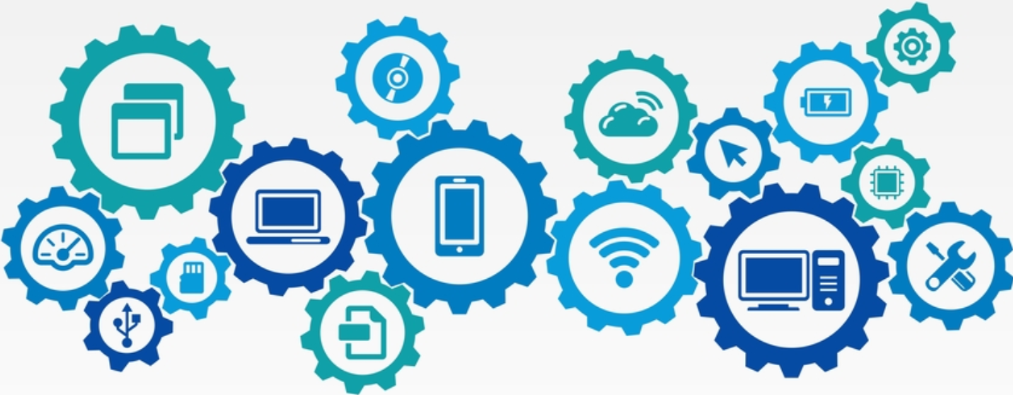
\includegraphics[width = \linewidth]{img/misc/integ.png}
        \caption{Intégration de système}%
        \label{fig:misc/integ}
    \end{figure}
\end{frame}

\subsection{Présentation de l'entreprise}

\begin{frame}
    \frametitle{Orange Cyberdéfense}
    \begin{minipage}{0.5\textwidth}
        \begin{itemize}
            \item Filiale d'Orange Business Services et du groupe Orange.
            \item Fondée en 2014, marque créée en 2016, 1100 employés.
            \item Fournit divers services de sécurité informatique.
        \end{itemize}
    \end{minipage}%
    \hfill
    \begin{minipage}{0.5\textwidth}
        \begin{figure}[h!]
            \centering
            
\includegraphics[width = \linewidth]{img/logo/ocd.png}
            \caption{Logo de l'entreprise}%
            \label{fig:logo/ocd}
        \end{figure}
    \end{minipage}
\end{frame}


\section{Mission}
\subsection{Objectifs}

\begin{frame}
    \frametitle{Objectifs}
    \begin{itemize}
        \item Apprendre en auto-formation.
        \item Concevoir et implémenter des architectures sécurisées.
        \item Élaborer des documentations techniques.
        \item Réaliser des projets pour des clients.
        \item Contribuer à des activités internes.
    \end{itemize}
\end{frame}

\subsection{Premières missions}

\begin{frame}
    \frametitle{Auto-formation}
    \begin{minipage}{0.6\textwidth}
        \begin{itemize}
            \item Montée en compétences sur les outils et technologies que
                j'allais utiliser par la suite.
            \item Fortinet:
            \begin{itemize}
                \item FortiGate,
                \item FortiManager,
                \item FortiAnalyzer;
            \end{itemize}
            \item Palo Alto Networks: PAN OS\@;
            \item Microsoft Azure.
        \end{itemize}
    \end{minipage}%
    \hfill
    \begin{minipage}{0.4\textwidth}
        \begin{figure}[h!]
            \centering
            
\includegraphics[width = 0.8\linewidth]{img/misc/self-learning.png}%
            \label{fig:misc/self-learning}
        \end{figure}
    \end{minipage}
\end{frame}

\begin{frame}
    \frametitle{Documentation de la salle de tests}
    \begin{minipage}{0.5\textwidth}
        \begin{itemize}
            \item Petite salle serveur pour des essais et de la pré-production.
            \item Revue des baies et équipements internes.
            \item Étiquetage des équipements et des câbles.
            \item Ajout de noms d'hôte et de descriptions d'interfaces.
            \item Inventaire complet des baies et de la réserve.
        \end{itemize}
    \end{minipage}%
    \hfill
    \begin{minipage}{0.45\textwidth}
        \begin{figure}[h!]
            \centering
            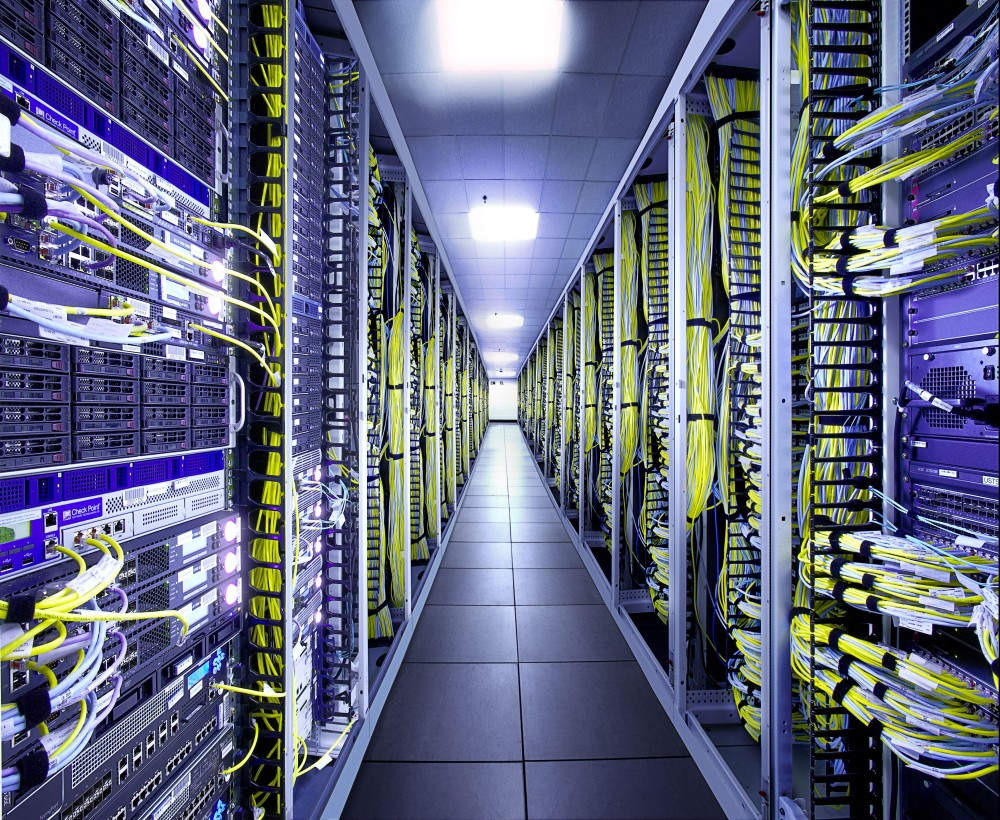
\includegraphics[width = \linewidth]{img/misc/data-center.jpg}
            \caption{Image non contractuelle}%
            \label{fig:misc/data-center}
        \end{figure}
    \end{minipage}
\end{frame}

\subsection{Deuxième mission: projet SNCF}

\begin{frame}
    \frametitle{Projet SCNF Access}
    \begin{itemize}
        \item Projet démarré début 2019 et en fin lorsque je le rejoins.
        \item Zone tampon entre l'Internet public et des services SNCF\@.
        \item Analyse avancée du trafic: pare-feu, WAF, IPS\@.
        \item Redondance: \textit{reverse proxy}, GRE, DNS, VIPs, liens croisés.
    \end{itemize}
\end{frame}

\begin{nohead}
    \begin{frame}
        \frametitle{Architecture}
        \begin{figure}[h!]
            \centering
            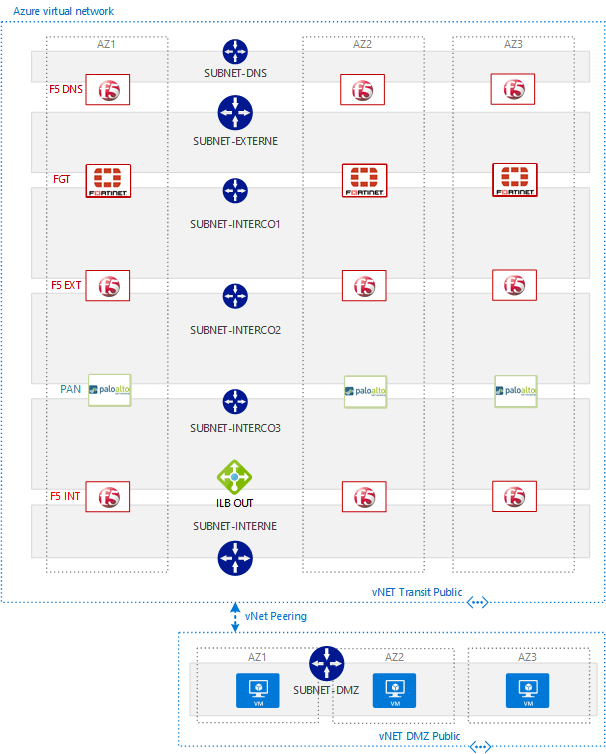
\includegraphics[height = 1.1\textheight]{img/sncf-access/arch.png}%
            \label{fig:sncf-access/arch}
        \end{figure}
    \end{frame}
\end{nohead}

\begin{frame}
    \frametitle{La mission}
    \begin{itemize}
        \item Rédaction d'un Dossier d'EXploitation (DEX).
        \item Plutôt guide d'implémentation de nouveaux services.
        \item Détail de toutes les actions à effectuer à chaque couche.
        \item Manipulation des infrastructures FortiGate et PAN OS en production
            pour aider à la rédaction.
    \end{itemize}
\end{frame}

\subsection{Mission principale: projet Hynamics}
\subsubsection{Considérations générales}

\begin{frame}
    \frametitle{Considérations générales}
    \begin{itemize}
        \item Filiale d'EDF fondée en avril 2019.
        \item Production de dihydrogène renouvelable et à basse émission de
            $CO_2$.
        \item Besoin de sécurité sur leur nouveaux sites: contact d'OCD\@.
        \item Sites concernés:
        \begin{itemize}
            \item La Défense (DEF): <<quartier général>>,
            \item Fontainebleau, <<Les Renardières>> (RNRD): plate-forme de
                test,
            \item Auxerre (AUXR): site de production.
        \end{itemize}
    \end{itemize}
\end{frame}

\begin{frame}
    \frametitle{Architecture globale}
    \begin{figure}[h!]
        \centering
        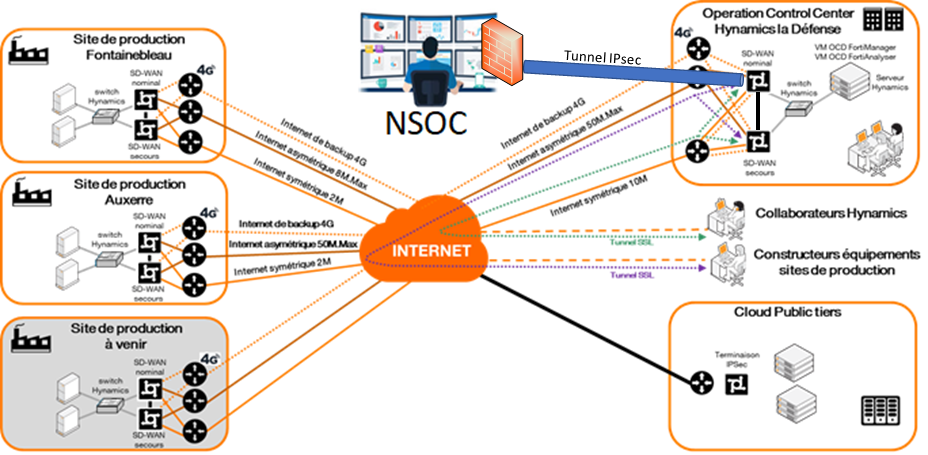
\includegraphics[width = 0.95\linewidth]{img/doc-hy/global-arch.png}
        \caption{Vue d'ensemble du projet}%
        \label{fig:doc-hy/global-arch}
    \end{figure}
\end{frame}

\begin{frame}
    \frametitle{Architecture physique}
    \begin{figure}[h!]
        \centering
        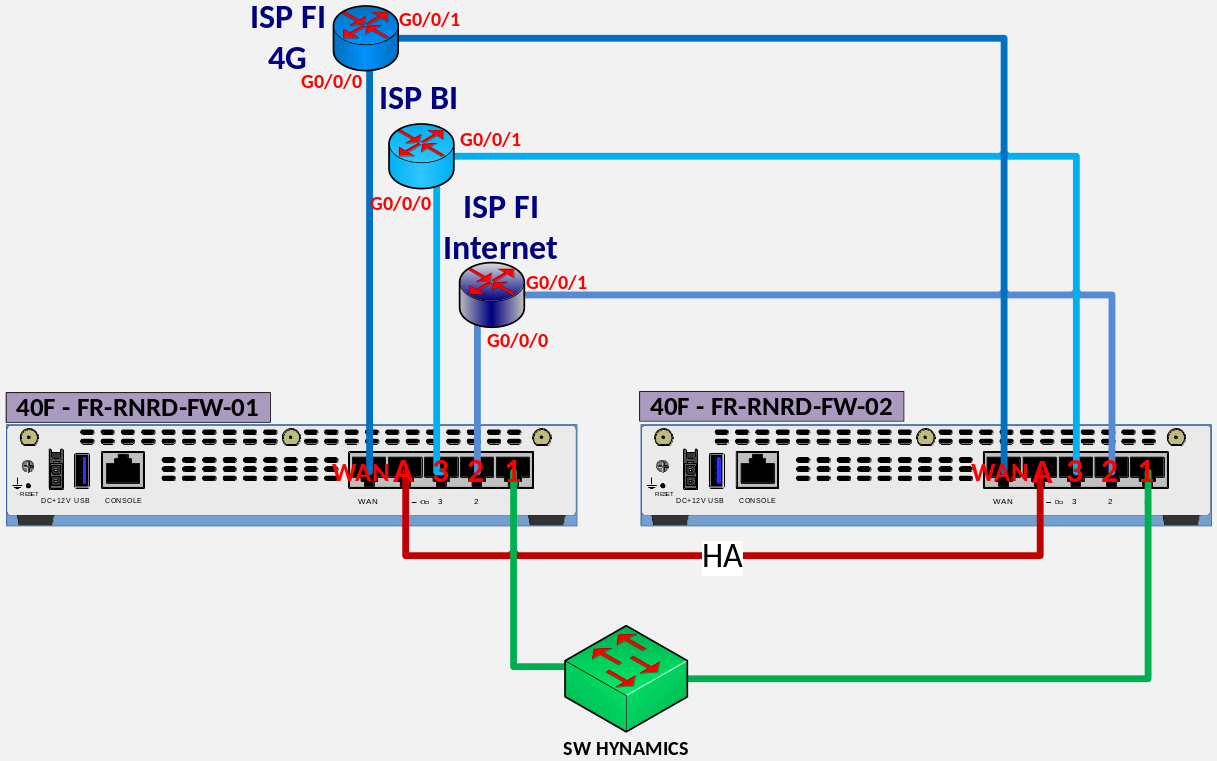
\includegraphics[width = 0.9\linewidth]{img/doc-hy/site-phys-arch.png}
        \caption{Pour le site de Fontainebleau}%
        \label{fig:doc-hy/site-phys-arch}
    \end{figure}
\end{frame}

\begin{frame}
    \frametitle{Architecture logique}
    \begin{figure}[h!]
        \centering
        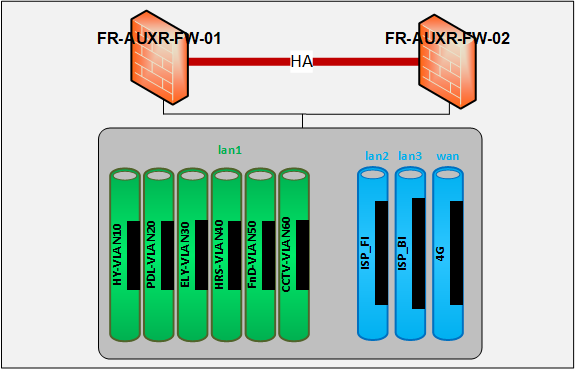
\includegraphics[width = 0.9\linewidth]{img/doc-hy/site-logi-arch.png}
        \caption{Pour le site d'Auxerre}%
        \label{fig:doc-hy/site-logi-arch}
    \end{figure}
\end{frame}

\subsubsection{Démarrage et premières opérations}

\begin{frame}
    \frametitle{Démarrage et premières opérations}
    \begin{itemize}
        \item Réunion de Lancement Interne (RLI) puis Externe (RLE).
        \item Ateliers techniques pour exliquer certains aspects au client et
            rassembler un maximum d'informations essentielles au projet.
        \item Achat, livraison et installation en salle de tests des pares-feux.
        \item Tests physiques et configuration des pares-feux pour avoir un
            accès d'administration à distance.
    \end{itemize}
\end{frame}

\begin{frame}
    \frametitle{VPN TLS \textit{vs.} Tunnel IPsec}
    \begin{figure}[h!]
        \centering
        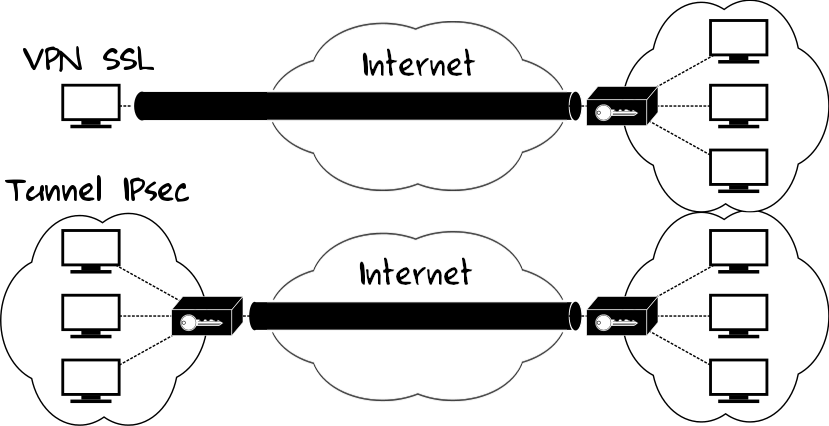
\includegraphics[width = \linewidth]{img/misc/tls-vs-ipsec.png}
        \caption{Fonctionnement typique}%
        \label{fig:misc/tls-vs-ipsec}
    \end{figure}
\end{frame}

\subsubsection{Collecte des informations et déploiement sur sites}

\begin{frame}
    \frametitle{Collecte des informations et déploiement sur sites}
    \begin{itemize}
        \item Interaction avec le client et ses partenaires au travers d'un
            <<fichier de collecte>>.
        \item Rédaction du Dossier de Spécifications Détaillées (DSD).
        \item Évolution de la configuration des pares-feux.
        \item Désinstallation et remballage des pares-feux pour livraison.
        \item Déploiement sur sites.
    \end{itemize}
\end{frame}

\subsubsection{Implémentation de la configuration}

\begin{frame}
    \frametitle{Implémentation de la configuration}
    \begin{minipage}{0.3\textwidth}
        \begin{figure}[h!]
            \centering
            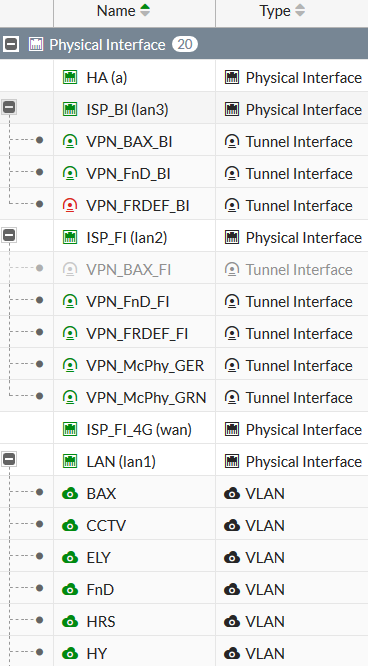
\includegraphics[width = \linewidth]{img/fgt-auxr/interfaces.png}
            \caption{Interfaces}%
            \label{fig:fgt-auxr/interfaces}
        \end{figure}
    \end{minipage}%
    \hfill
    \begin{minipage}{0.6\textwidth}
        \begin{figure}[h!]
            \centering
            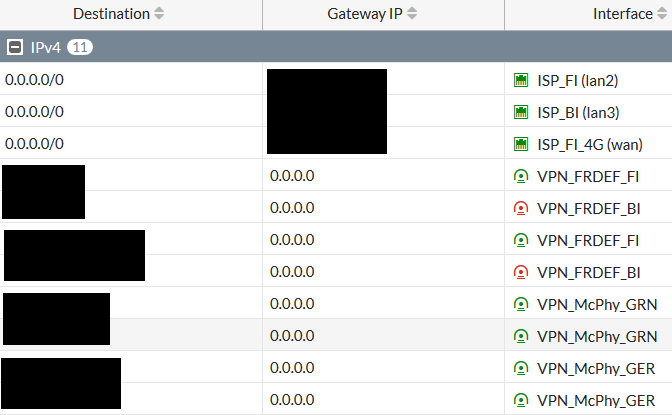
\includegraphics[width = \linewidth]{img/fgt-auxr/routes.png}
            \caption{Routes}%
            \label{fig:fgt-auxr/routes}
        \end{figure}
    \end{minipage}
\end{frame}

\begin{frame}
    \frametitle{Tunnels IPsec}
    \begin{minipage}{0.5\textwidth}
        \begin{figure}[h!]
            \centering
            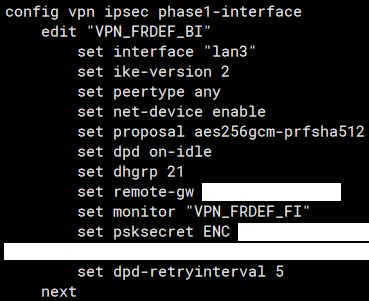
\includegraphics[width = \linewidth]{img/fgt-auxr/ipsec-phase1.png}
            \caption{Phase 1}%
            \label{fig:fgt-auxr/ipsec-phase1}
        \end{figure}
    \end{minipage}%
    \hfill
    \begin{minipage}{0.4\textwidth}
        \begin{figure}[h!]
            \centering
            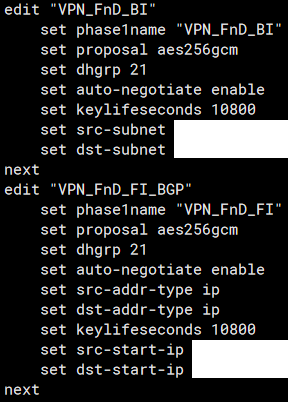
\includegraphics[width = \linewidth]{img/fgt-auxr/ipsec-phase2.png}
            \caption{Phases 2}%
            \label{fig:fgt-auxr/ipsec-phase2}
        \end{figure}
    \end{minipage}
\end{frame}

\begin{frame}
    \frametitle{BGP --- Voisins}
    \begin{minipage}{0.6\textwidth}
        \begin{figure}[h!]
            \centering
            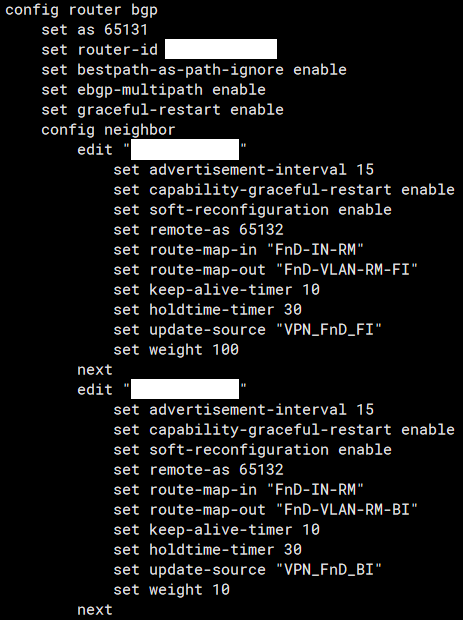
\includegraphics[height = 0.85\textheight]
                {img/fgt-auxr/bgp-neighbors.png}
            \caption{Configuration principale}%
            \label{fig:fgt-auxr/bgp-neighbors}
        \end{figure}
    \end{minipage}%
    \hfill
    \begin{minipage}{0.3\textwidth}
        \begin{figure}[h!]
            \centering
            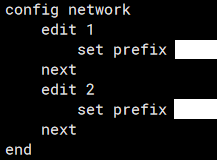
\includegraphics[width = \linewidth]{img/fgt-auxr/bgp-nets.png}
            \caption{Réseaux distribués}%
            \label{fig:fgt-auxr/bgp-nets}
        \end{figure}
    \end{minipage}
\end{frame}

\begin{frame}
    \frametitle{BGP --- Filtres}
    \begin{minipage}{0.55\textwidth}
        \begin{figure}[h!]
            \centering
            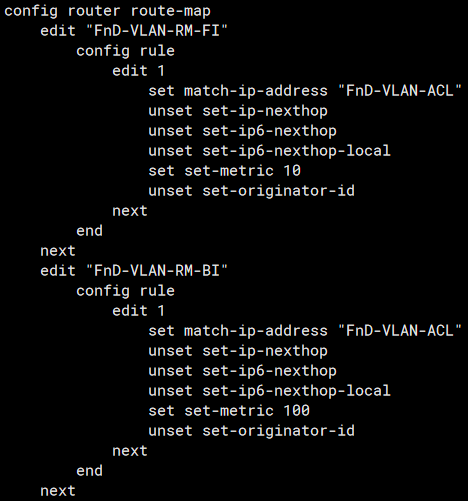
\includegraphics[width = \linewidth]{img/fgt-auxr/route-maps.png}
            \caption{Associations de routes}%
            \label{fig:fgt-auxr/route-maps}
        \end{figure}
    \end{minipage}%
    \hfill
    \begin{minipage}{0.4\textwidth}
        \begin{figure}[h!]
            \centering
            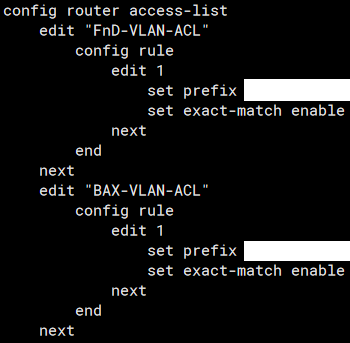
\includegraphics[width = \linewidth]{img/fgt-auxr/acl.png}
            \caption{Listes d'accès}%
            \label{fig:fgt-auxr/acl}
        \end{figure}
    \end{minipage}
\end{frame}

\begin{frame}
    \frametitle{FortiManager}
    \framesubtitle{\textit{Policy Packages}}
    \begin{figure}[h!]
        \centering
        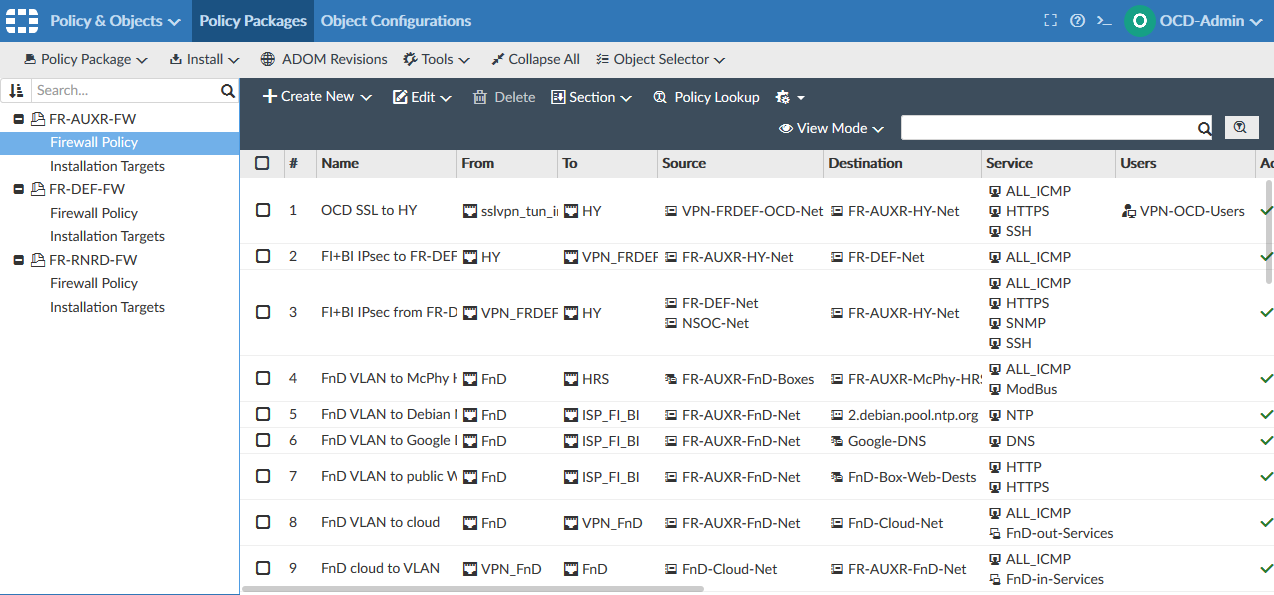
\includegraphics[height = 0.65\textheight]{img/fmg/policy-packages.png}
        \caption{Pour le site d'Auxerre}%
        \label{fig:fmg/policy-packages}
    \end{figure}
\end{frame}

\begin{frame}
    \frametitle{FortiManager}
    \framesubtitle{Associations groupe d'utilisateurs --- portail VPN}
    \begin{figure}[h!]
        \centering
        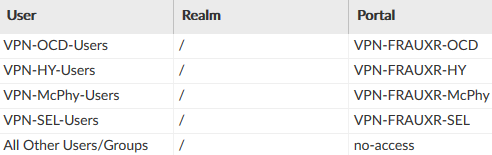
\includegraphics[width = \linewidth]{img/fmg/ssl-mappings.png}
        \caption{Pour le site d'Auxerre}%
        \label{fig:fmg/ssl-mappings}
    \end{figure}
\end{frame}

\begin{frame}
    \frametitle{FortiManager}
    \framesubtitle{Portail VPN}
    \begin{figure}[h!]
        \centering
        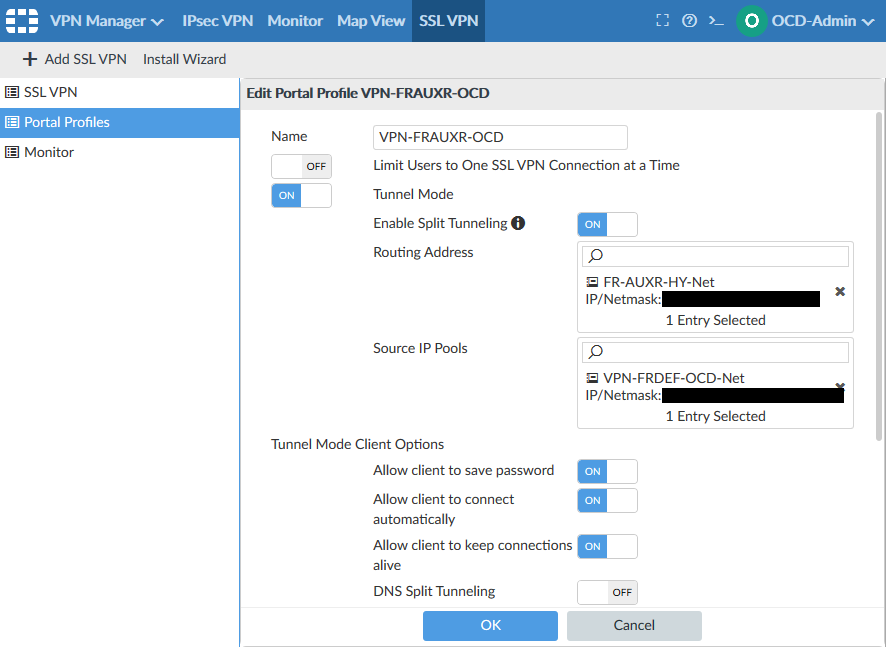
\includegraphics[width = 0.8\linewidth]{img/fmg/ssl-portal.png}
        \caption{Pour les utilisateurs Hynamics sur Auxerre}%
        \label{fig:fmg/ssl-portal}
    \end{figure}
\end{frame}

\subsubsection{Mise en place des tests et migration}

\begin{frame}
    \frametitle{Mise en place des tests et migration}
    \begin{itemize}
        \item Préparation d'un Dossier de Tests de Validation (DTV) par site.
        \item Réalisation d'une Vérification d'Aptitude au Bon Fonctionnement
            (VABF) par site en suivant son DTV associé:
        \begin{itemize}
            \item La Défense: pas de souci particulier;
            \item Fontainebleau: mis de côté;
            \item Auxerre: majoritairement bien, mais quelques soucis:
            \begin{itemize}
                \item Commutateur incapable de gérer les VLANs;
                \item BGP défectueux avec un partenaire;
                \item Manque de retour d'un autre partenaire sur ses tests
                    métiers suite à la fin de la VABF\@.
            \end{itemize}
        \end{itemize}
    \end{itemize}
\end{frame}

\subsubsection{Transferts de connaissances}

\begin{frame}
    \frametitle{Transferts de connaissances}
    \framesubtitle{Assurer le bon déroulement de la suite du projet}
    \begin{minipage}{0.5\textwidth}
        \begin{itemize}
            \item Pour:
            \begin{itemize}
                \item L'ingénieur \textit{Run} chargé de la continuité du projet.
                \item Une nouvelle stagiaire chargée de la fin du \textit{Build}.
            \end{itemize}
            \item Contenu:
            \begin{itemize}
                \item Vue d'ensemble du projet, de ses objectifs et de ses
                    contraintes.
                \item Plus dans les détails pour ce qui concerne directement la
                    personne en question.
            \end{itemize}
        \end{itemize}
    \end{minipage}%
    \hfill
    \begin{minipage}{0.4\textwidth}
        \begin{figure}[h!]
            \centering
            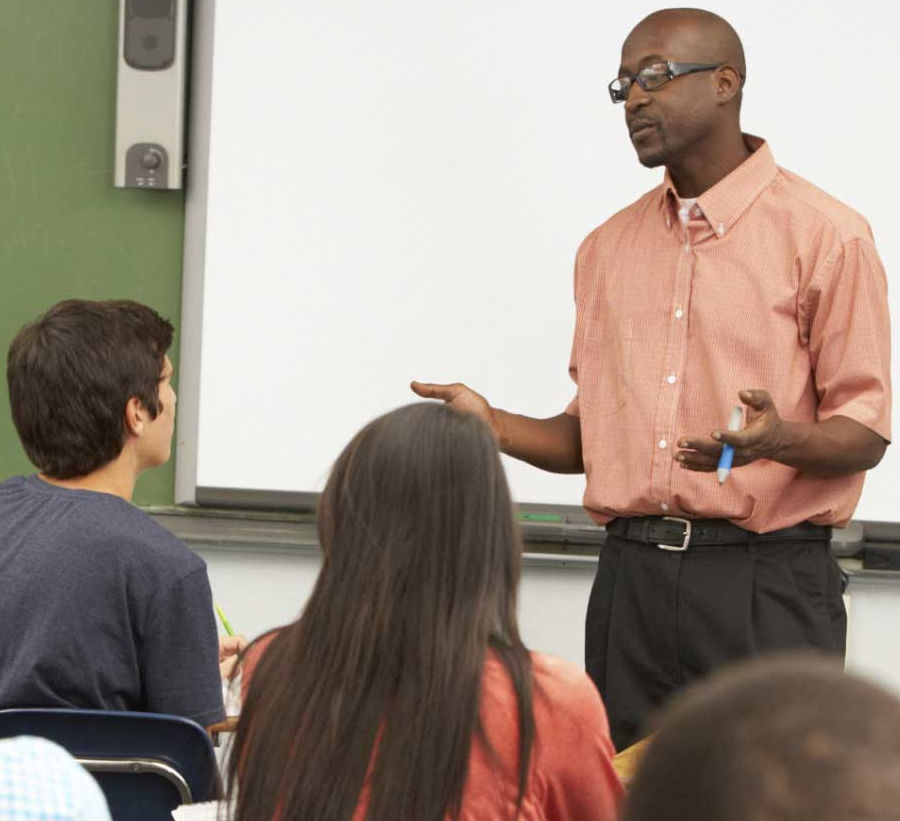
\includegraphics[width = \linewidth]{img/misc/teacher.jpg}%
            \label{fig:misc/teacher}
        \end{figure}
    \end{minipage}
\end{frame}


\section{Bilan}

\begin{frame}
    \frametitle{Bilan}
    \begin{itemize}
        \item Stage chez un prestataire de services: principalement des projets
            client.
        \item Projet Hynamics:
        \begin{itemize}
            \item Leur permet d'avoir une production en place.
            \item Ils peuvent commencer à servir leurs clients.
            \item Certaines choses n'ont pas pu être terminées.
            \item Bons retours de leur part.
        \end{itemize}
    \end{itemize}
\end{frame}

\subsection{Retour d'expérience}

\begin{frame}
    \frametitle{Retour d'expérience}
    \begin{itemize}
        \item Points positifs:
        \begin{itemize}
            \item Entreprise spécialisée en sécurité.
            \item Découverte de l'intégration et du \textit{Build}.
            \item Pratique et maîtrise de nouvelles technologies.
        \end{itemize}
        \item Points négatifs:
        \begin{itemize}
            \item Manque de participation à la conception: <<juste configurer>>.
            \item Par conséquent, certaines tâches étaient assez répétitives.
            \item Petites équipes projet donc peu de cohésion globale.
            \item Le télétravail scinde encore un peu plus.
        \end{itemize}
    \end{itemize}
\end{frame}


\section{Conclusion}
\subsection{Perspectives}


\end{document}
